%
% teil5.tex -- Beispiel-File für Teil 5
%
% (c) 2020 Prof Dr Andreas Müller, Hochschule Rapperswil
%
% !TEX root = ../../buch.tex
% !TEX encoding = UTF-8
%
\section{Rücktransformation (ICWT)
\label{wavelets:section:teil5}}
\kopfrechts{Rücktransformation (ICWT)}

In diesem kurzen Abschnitt wird die Rücktransformation vom Frequenz-
in den Zeitbereich betrachtet.
Dabei wird die erhaltene $a_n \times b_m$ Matrix (aus der CWT),
welche die Transformationsparameter im Bildbereich beinhaltet, in
den Zeitbereich rücktransformiert.
Dabei sollte in dieser Betrachtung wieder das Ausgangssignal aus
der Abbildung \ref{wavelet:fig:FFTnoiseFree} zurück gewonnen werden.
Das erhaltene Resultat aus der ICWT Abbildung \ref{wavelet:fig:ICWT},
entpricht aber nicht wirklich dem eingangs transformierten Signal,
weil:

\begin{itemize}
	\item die CWT ein verschmiertes Spektrum erzeugt.
	\item das Morlet-Wavelet einem gaussgewichteten Cosinus
	entspricht und damit kein scharfkantiges Sinus- oder
	Cosinussignal reproduziert werden kann.
\end{itemize}

Um letztere These genauer zu untersuchen, wurden zwei Wege eingeschlagen.
Zum einen die Rücktransformation des Cosinus über dasselbe Gauss-Fenster
mit dem schon das Wavelet generiert wurde und zum Anderen mit einem
Rechteckfenster, in der Hoffnung, dass dieses ein reines Sinussignal
besser reproduzieren kann.

Abbildung \ref{wavelet:fig:ICWT} zeigt aber, dass die Problematik
in erster Linie beim Verschmieren der Frequenzausgabe liegt.
Die CWT detektiert die Frequenz nicht gleich scharf wie die FFT und
dadurch werden Frequenzen nahe der Hauptfrequenz ebenfalls mit einer
nennenswerten Amplitude im Frequenzspektrum angegeben.
Bei Rücktransformation werden diese Anteile mit einbezogen und
verursachen eine Überlagerung (analog zur Abbildung
\ref{wavelet:fig:AmplitudengangExtraktionDFT} unten).
Diese Störung verhindert Hauptsächlich die Möglichkeit mit der CWT eine sinnvolle Rücktransformation zu erhalten.
Aus Zeitgründen konnten hier auch keine weiteren Versuche für eine
Optimierung gestartet werden.
In gemachten ICWT wurde die Mittlung noch vernachlässigt, wodurch
die Amplitudenwerte durch die Aufsummierung der einzelnen spektralen
Anteile stark überhöht sind.

\begin{figure}
	\centering
	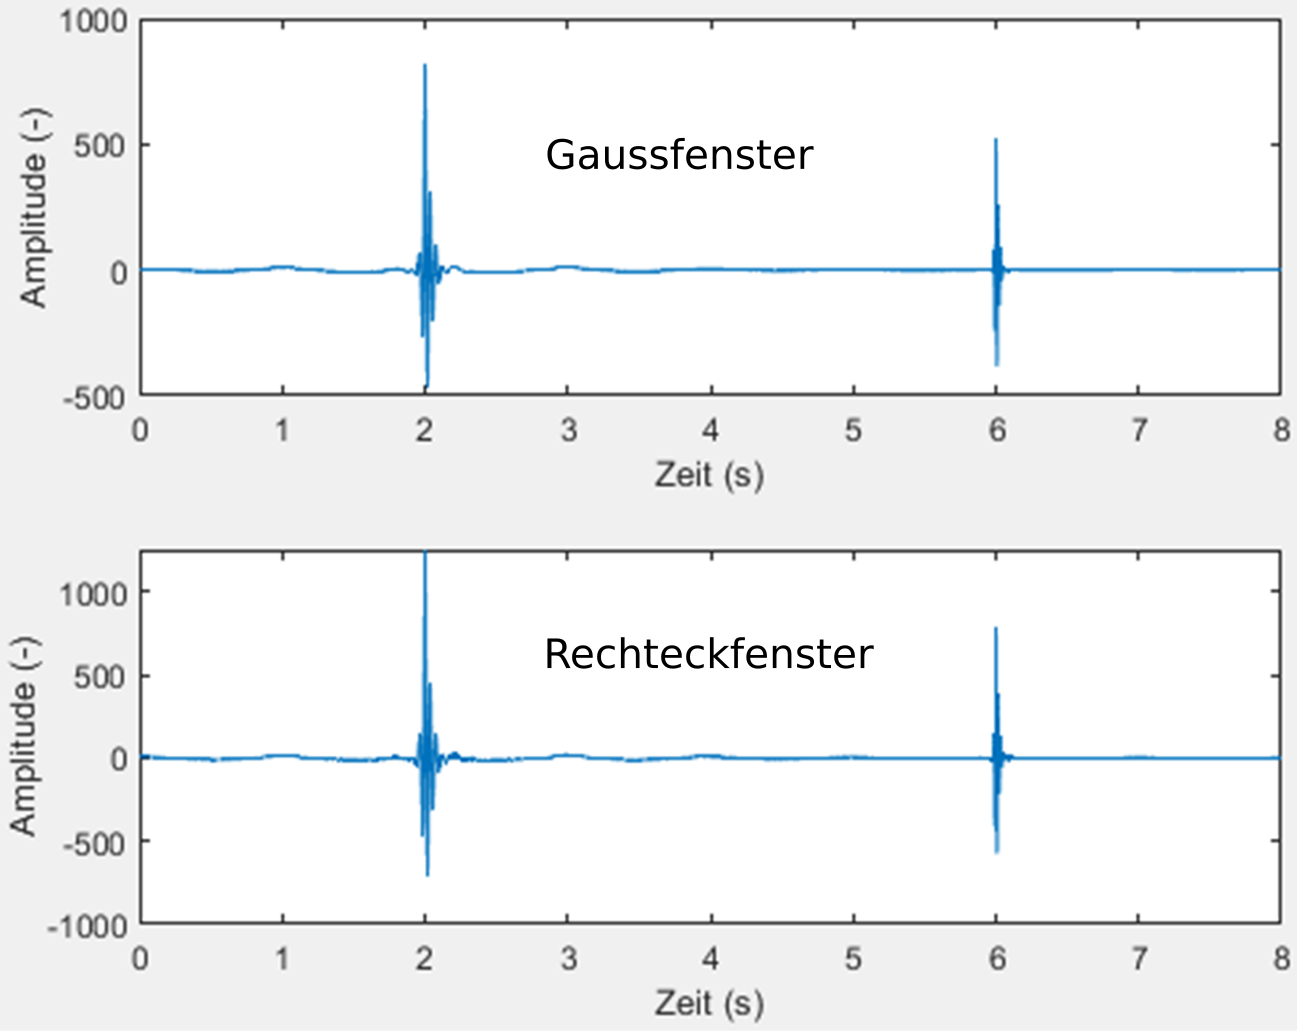
\includegraphics[width=0.75\textwidth]{papers/wavelets/images/19-1_ICWT.png}
	\caption{Rücktransformation des CWT-transformierten Testsignal
	aus Abbildung \ref{wavelet:fig:FFTnoiseFree}.
	Einerseits mit dem gaussschen Fenster, welches schon für die Erzeugung
	des Wavelets genutzt wurde.
	Andererseits mit einem Rechteckfenster.
	D.~h.~die durch die CWT erhaltene Transformationsmatrix
	$a_n \times b_m$, wird vom Bild in den Zeitbereich zurück
	transferiert.
	Die beiden Fenster stehen hierbei sinnbildlich dafür, ob
	eine reine Cosinuswelle (Rechteckfenster) oder ein Wavelet
	(Gauss-Fenster) mit den Bildmatrixparametern bestückt wird.
	Es zeigt sich, dass beide Varianten aufgrund der Verschmierung
	durch die CWT keine sinnvolle Rücktransformationen in den
	Zeitbereich ermöglichen.}
	\label{wavelet:fig:ICWT}
\end{figure}
